% ============================================================
% 05_arquitectura.tex
% ============================================================

\section{Arquitectura y Diseño de la Solución}
\label{sec:arquitectura}

\subsection{Arquitectura general del sistema}

NodeAlert IoT adopta una arquitectura IoT de tres capas: capa de percepción
(nodo sensor embebido), capa de comunicación (red Wi-Fi y broker MQTT) y capa
de aplicación (backend Node-RED, base de datos SQLite y frontend web). La
Figura~\ref{fig:arquitectura} ilustra esta organización.

\begin{figure}[htbp]
  \centering
  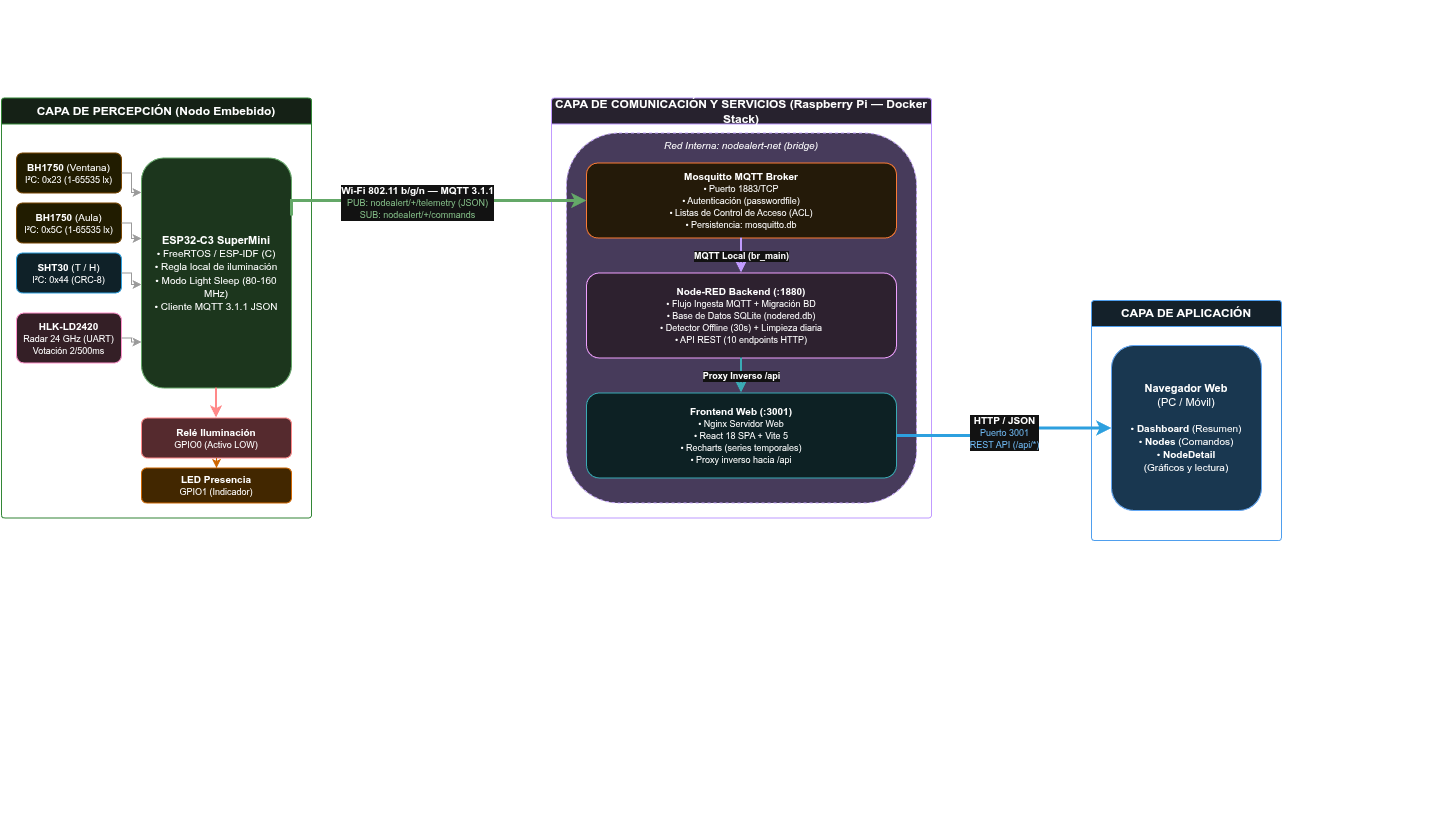
\includegraphics[width=0.95\textwidth]{figuras/arquitectura_general.png}
  \caption{\textit{Arquitectura general de NodeAlert IoT con sus tres capas: percepción, comunicación y aplicación.}}
  \label{fig:arquitectura}
\end{figure}

\subsection{Nodo sensor: arquitectura del firmware}

El firmware del nodo está diseñado en torno al bucle principal de la función
\texttt{app\_main}, que ejecuta en el contexto de la tarea principal de FreeRTOS.
La arquitectura evita la creación de tareas adicionales, manteniendo una única
tarea de ejecución que opera en un ciclo de 20\,ms. La Figura~\ref{fig:fw_bloques}
ilustra el diagrama de bloques del firmware.

\begin{figure}[htbp]
  \centering
  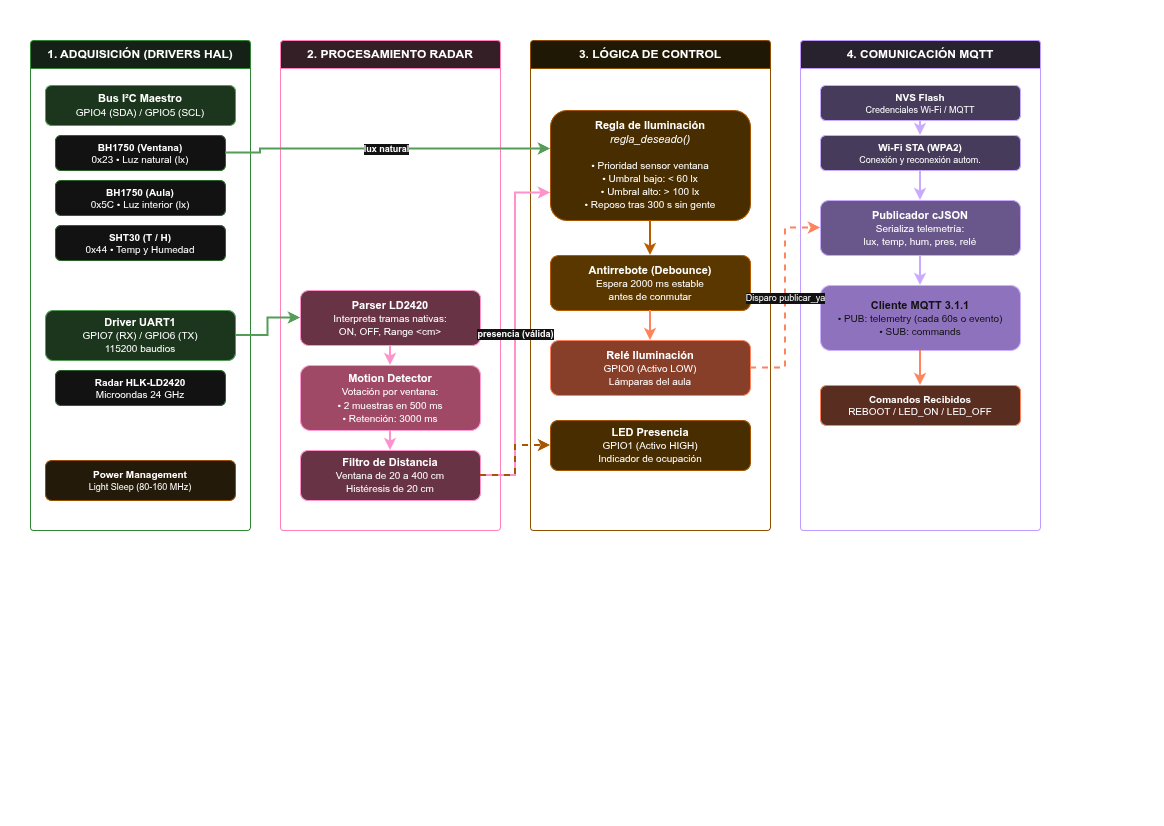
\includegraphics[width=0.95\textwidth]{figuras/firmware_bloques.png}
  \caption{\textit{Diagrama de bloques del firmware del nodo ESP32-C3.}}
  \label{fig:fw_bloques}
\end{figure}

\subsubsection{Módulo de sensores I\textsuperscript{2}C}

Los tres dispositivos I\textsuperscript{2}C (dos BH1750 y el SHT30) comparten el
bus I2C0 inicializado mediante el driver \texttt{i2c\_master} de ESP-IDF. Las
lecturas se realizan cada 1000\,ms. Cada driver implementa reconexión automática:
ante un fallo de comunicación, el dispositivo se marca como no disponible y se
reintenta la inicialización cada 30\,s. Esta estrategia de recuperación elástica
garantiza que la lógica de control continúe operando aunque uno o más sensores
fallen temporalmente.

\subsubsection{Módulo del radar LD2420}

El driver del radar LD2420 implementa en su totalidad el modo de reporte nativo
simple. Al inicializar, envía la secuencia de comandos binaria que configura el
módulo en este modo, con tramas delimitadas por los bytes \texttt{FD FC FB FA} y
\texttt{04 03 02 01}. El parser de líneas acumula los bytes UART en un buffer de
24 caracteres e interpreta los mensajes de texto emitidos.

Sobre el parser se ejecuta un detector de movimiento con lógica de votación que
requiere un mínimo de dos evidencias válidas en una ventana de 500\,ms para activar
la señal de presencia (\textit{required\_evidence} = 2,
\textit{evidence\_window} = 500\,ms). Una vez activada, la señal se mantiene
durante 3\,s adicionales sin nuevas evidencias (\textit{hold\_ms} = 3000). El
estado se declara obsoleto (\textit{stale}) si no se reciben datos en más de 1\,s.

\subsubsection{Lógica de control de iluminación}

La función de control de iluminación se implementó como una función pura sin
efectos secundarios en el archivo \texttt{regla\_luz.h}, siguiendo el principio
de separación entre lógica y hardware. La función \texttt{regla\_deseado()} recibe
como parámetros el estado actual del sistema, la disponibilidad y valores de los
sensores de luz, el estado actual del relé y los umbrales de iluminación, y
devuelve el estado deseado del relé.

La Figura~\ref{fig:diagrama_regla} ilustra el diagrama de flujo de la lógica de
control.

\begin{figure}[htbp]
  \centering
  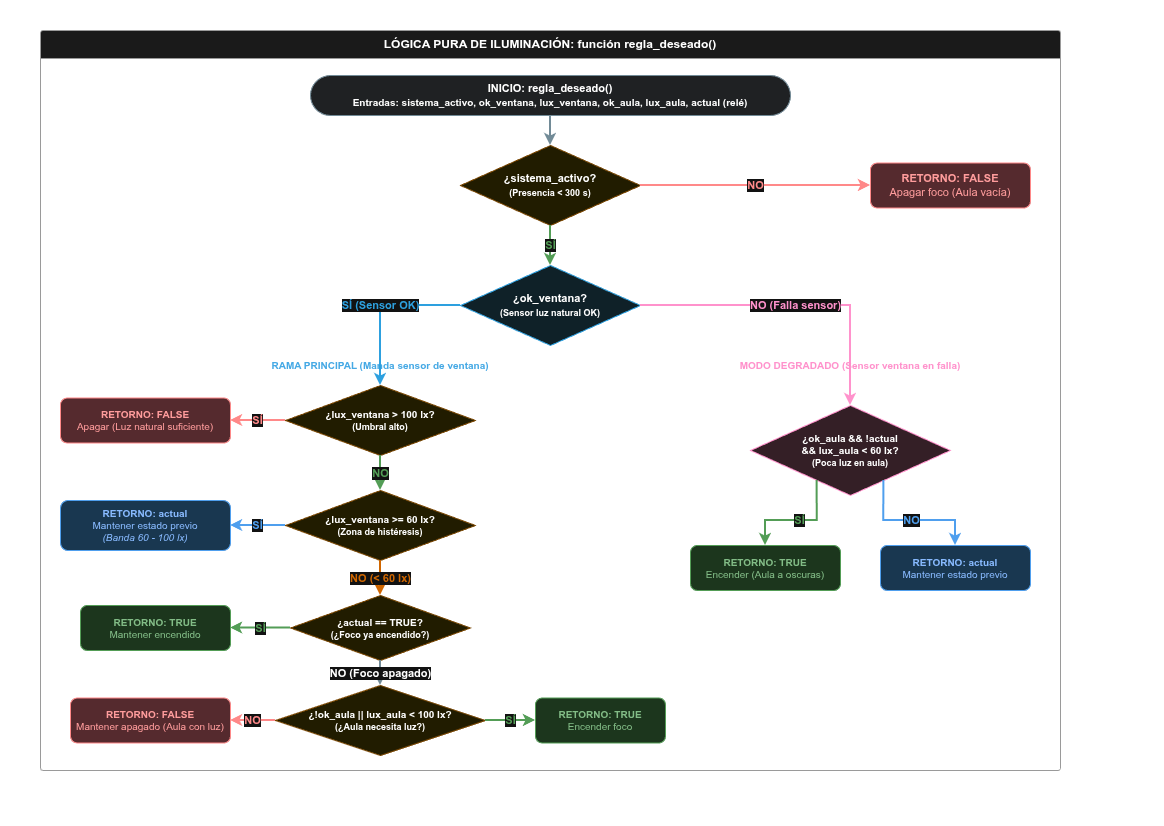
\includegraphics[width=0.88\textwidth]{figuras/diagrama_flujo_regla.png}
  \caption{\textit{Diagrama de flujo de la función \texttt{regla\_deseado()}: lógica de control de iluminación con histéresis de doble umbral.}}
  \label{fig:diagrama_regla}
\end{figure}

El debounce por software de 2\,s actúa en la capa de control del relé
(\texttt{controlar\_rele()}): un cambio de estado del relé solo se ejecuta si el
estado deseado se mantiene estable durante al menos 2000\,ms, evitando oscilaciones
ante variaciones bruscas de luminosidad.

\subsection{Arquitectura del servidor}

La Figura~\ref{fig:docker_arch} muestra la arquitectura de contenedores Docker.

\begin{figure}[htbp]
  \centering
  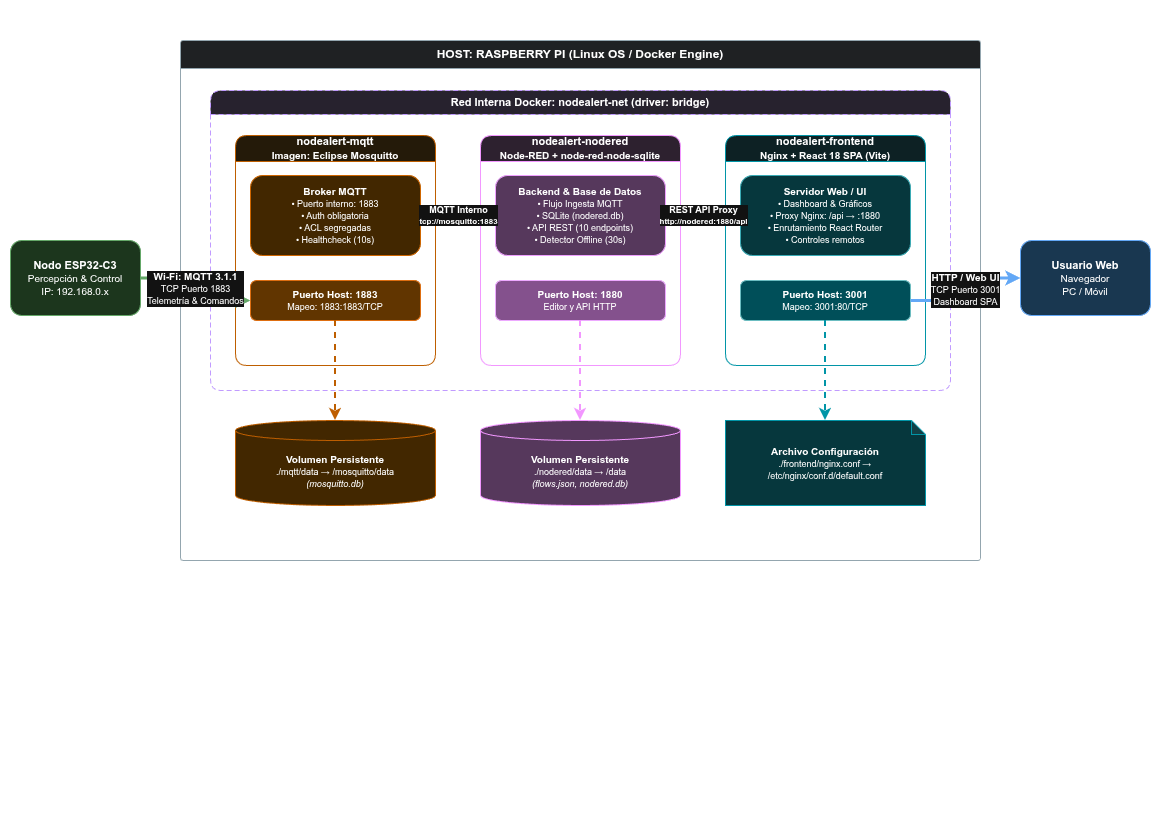
\includegraphics[width=0.95\textwidth]{figuras/docker_arquitectura.png}
  \caption{\textit{Arquitectura de contenedores Docker desplegada en Raspberry Pi. Los tres servicios se comunican a través de la red interna \texttt{nodealert-net}.}}
  \label{fig:docker_arch}
\end{figure}

\subsubsection{Esquema de base de datos SQLite}

Node-RED persiste todos los datos de telemetría en una base de datos SQLite local
(\texttt{nodered.db}). El esquema comprende tres tablas principales:

\begin{itemize}
  \item \textbf{nodes}: registro de nodos conocidos con campos \texttt{node\_id}
        (PK), \texttt{name}, \texttt{is\_online}, \texttt{last\_seen} y
        \texttt{hidden}.
  \item \textbf{telemetry}: serie temporal de mediciones con campos para
        temperatura, gas, llama, estado de presencia, iluminancia ventana/aula,
        temperatura interna, humedad y estado del relé, con índice sobre
        (\texttt{node\_id}, \texttt{timestamp}).
  \item \textbf{node\_config}: configuración por nodo (umbrales de temperatura,
        gas, llama) con valores predeterminados.
\end{itemize}

La tabla \texttt{telemetry} implementa un mecanismo de migraciones en cadena
ejecutado en el flujo \textit{Init DB} de Node-RED, que verifica la existencia de
cada columna antes de agregarla mediante \texttt{ALTER TABLE}, garantizando
compatibilidad hacia adelante.

\subsection{Tópicos MQTT}

La comunicación MQTT utiliza el espacio de nombres jerárquico
\texttt{nodealert/<device\_id>/\{telemetry | commands\}}, donde
\texttt{<device\_id>} es el identificador único del nodo (por ejemplo,
\texttt{nodealert-luz01}). La Tabla~\ref{tab:mqtt_topics} resume los tópicos
utilizados.

\begin{table}[htbp]
  \caption{\textit{Tópicos MQTT del sistema NodeAlert IoT.}}
  \label{tab:mqtt_topics}
  \centering
  \small
  \begin{tabularx}{\textwidth}{@{}llX@{}}
    \toprule
    \textbf{Tópico} & \textbf{QoS} & \textbf{Descripción} \\
    \midrule
    \texttt{nodealert/+/telemetry} & 1 & Telemetría JSON publicada por el nodo cada 60\,s o ante evento \\
    \texttt{nodealert/<id>/commands} & 1 & Comandos de texto enviados desde el servidor al nodo \\
    \bottomrule
  \end{tabularx}
  \vspace{4pt}

  \noindent\textit{Nota.} El símbolo \texttt{+} en el tópico de suscripción de Node-RED es
  un comodín de un nivel que permite recibir telemetría de todos los nodos registrados.
\end{table}

\subsection{API REST}

Node-RED expone una API REST HTTP sobre el puerto 1880 que el frontend React consume
mediante solicitudes Axios. La Tabla~\ref{tab:api_endpoints} lista los endpoints
implementados.

\begin{table}[htbp]
  \caption{\textit{Endpoints de la API REST expuesta por Node-RED.}}
  \label{tab:api_endpoints}
  \centering
  \small
  \begin{tabularx}{\textwidth}{@{}llX@{}}
    \toprule
    \textbf{Método} & \textbf{Endpoint} & \textbf{Descripción} \\
    \midrule
    GET  & \texttt{/api/health}                     & Estado del servicio \\
    GET  & \texttt{/api/nodes}                      & Lista de nodos visibles \\
    GET  & \texttt{/api/nodes/:id}                  & Detalle de nodo con última telemetría \\
    POST & \texttt{/api/nodes}                      & Registrar nodo manualmente \\
    DELETE & \texttt{/api/nodes/:id}                & Ocultar nodo (soft delete) \\
    GET  & \texttt{/api/telemetry/latest}           & Última telemetría de todos los nodos \\
    GET  & \texttt{/api/telemetry/:id}              & Historial de telemetría de un nodo \\
    GET  & \texttt{/api/telemetry/averages}         & Promedios de la última hora \\
    GET  & \texttt{/api/nodes/:id/config}           & Configuración del nodo \\
    POST & \texttt{/api/nodes/:id/command}          & Publicar comando vía MQTT \\
    \bottomrule
  \end{tabularx}
  \vspace{4pt}

  \noindent\textit{Nota.} El endpoint \texttt{POST /api/nodes/:id/config} devuelve
  HTTP 405, dado que los umbrales operativos son parámetros de compilación del firmware.
\end{table}

